%% Figure from MATH 556 notes, section 49 (Lecture 22). ADDED (not from lecture).
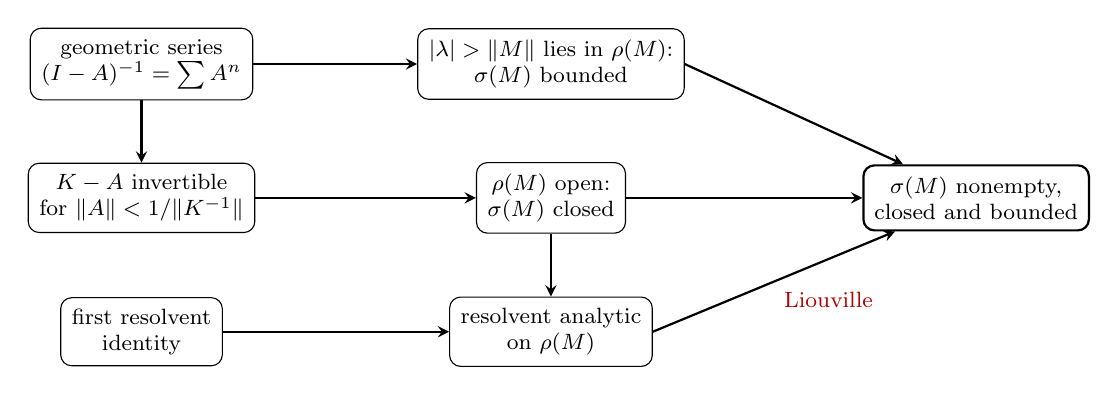
\begin{tikzpicture}[>=stealth, every node/.style={font=\footnotesize}]
    \node[draw, rounded corners, align=center, inner sep=4pt] (a) at (0,1.7) {geometric series\\$(I - A)^{-1} = \sum A^n$};
    \node[draw, rounded corners, align=center, inner sep=4pt] (d) at (5.2,1.7) {$|\lambda| > \|M\|$ lies in $\rho(M)$:\\$\sigma(M)$ bounded};
    \node[draw, rounded corners, align=center, inner sep=4pt] (b) at (0,0) {$K - A$ invertible\\for $\|A\| < 1/\|K^{-1}\|$};
    \node[draw, rounded corners, align=center, inner sep=4pt] (c) at (5.2,0) {$\rho(M)$ open:\\$\sigma(M)$ closed};
    \node[draw, rounded corners, align=center, inner sep=4pt] (g) at (0,-1.7) {first resolvent\\identity};
    \node[draw, rounded corners, align=center, inner sep=4pt] (e) at (5.2,-1.7) {resolvent analytic\\on $\rho(M)$};
    \node[draw, thick, rounded corners, align=center, inner sep=4pt] (f) at (10.6,0) {$\sigma(M)$ nonempty,\\closed and bounded};
    \draw[->, thick] (a) -- (d);
    \draw[->, thick] (a) -- (b);
    \draw[->, thick] (b) -- (c);
    \draw[->, thick] (c) -- (e);
    \draw[->, thick] (g) -- (e);
    \draw[->, thick] (c) -- (f);
    \draw[->, thick] (d.east) -- (f);
    \draw[->, thick] (e.east) -- node[below right, red!70!black] {Liouville} (f);
\end{tikzpicture}
